\documentclass[12pt]{article}
\usepackage[utf8]{inputenc}
\usepackage{sbc-template}
\usepackage{placeins}

\usepackage{graphicx,url}

\usepackage[brazil]{babel}   
%\usepackage[latin1]{inputenc}  

     
\sloppy

\title{Saúde do Trabalhador\\Padrões em Afastamentos e Desligamentos}

\author{Ivair Nobrega Luques\inst 1}


\address{Centro Federal de Educação Tecnológica Celso Suckow da Fonseca - CEFET-RJ
 \email{ ivair.luques@eic.cefet-rj.br }
}

\begin{document} 

\maketitle

     
\begin{resumo} 
  Planejar ações eficazes na garantia dos direitos da Saúde do Trabalhador é uma tarefa de grande complexidade. 
  Extrair informações das bases de dados públicas, que apoiem a tomada de decisão dos gestores de instituições de defesa dos trabalhadores é essencial.
  Padrões Frequentes é uma metodologia de Mineração de Dados utilizada para verificar a existência de padrões em um conjunto de dados. O algoritmo a ser aplicado neste trabalho é o Apriori que tem por objetivo identificar regras de associação entre as diferentes classes de informação disponibilizadas.
  \end{resumo}


\section{Introdução}

``No ano de 1985, o número de acidentes de trabalho, segundo os dados oficiais da previdência social, foi de 1.077.861 casos, com 4.384 mortes, uma média de mais de 12 mortes por dia. E eu começava a entender que o acidente de trabalho era um gravíssimo problema de saúde pública, negligenciado, até hoje, como tal." \cite{Vasconcellos2007}.

A questão da saúde do trabalhador não se restringe ao acompanhamento dos acidentes de trabalho:

``A área de Saúde do Trabalhador, no Brasil, tem uma conotação própria, reflexo da trajetória que lhe deu origem e vem constituindo seu marco referencial, seu corpo conceitual e metodológico. A princípio é uma meta, um horizonte, uma vontade que entrelaça trabalhadores, profissionais de serviços, técnicos e pesquisadores sob premissas nem sempre explicitadas."\cite{minayo1997construccao}

Dentro deste cenário de complexidade, é fundamental obter uma visão mais clara das relações entre os diversos fatores que o compõem, através dos dados oficiais divulgados.

Em 1985, após a oitava Conferência Nacional de Saúde, foi realizada a primeira Conferência Nacional da Saúde do Trabalhador. Uma das ações realizadas posteriormente foi a criação do Centro de Estudos da Saúde do Trabalhador e Ecologia Humana (Cesteh), em 10 de dezembro de 1985, que  integra a estrutura da Escola Nacional de Saúde Pública Sérgio Arouca (Ensp), da Fundação Oswaldo Cruz (Fiocruz).

O Cesteh atua nas áreas de Saúde, Trabalho e Ambiente, desenvolvendo atividades de Ensino, Pesquisa e Serviço.
A área de Ensino é responsável pela formação de recursos humanos para o campo da Saúde do Trabalhador e Ecologia Humana. Por meio de cursos de pós-graduação e estágios, o Cesteh forma pesquisadores, professores e técnicos para atuação e fortalecimento do campo da Saúde do Trabalhador, no âmbito do SUS e de outras instituições.\cite{Silva2000}

O Cesteh desenvolve pesquisas de caráter integrador e interdisciplinar abordando temas tradicionais no campo, como estudos clássicos em setores industriais que geram exposição com risco à saúde dos trabalhadores e consequências socioambientais (benzeno, amianto, mercúrio, chumbo, agrotóxicos, entre outros), além de pesquisas sobre relações de produção e gênero, formação e comunicação em saúde do trabalhador, saúde de profissionais da saúde e da educação, até temas emergentes como nanotecnologia, cronobiologia, alterações genéticas e desastres ambientais.

No Serviço, o Cesteh conta com o Ambulatório de Saúde do Trabalhador e o Laboratório de Toxicologia como referências no campo da Saúde do Trabalhador. Esses estão articulados com outros setores das políticas públicas e da sociedade para enfrentar os problemas e doenças relacionadas ao trabalho. Seus profissionais, com formação em diferentes áreas do conhecimento, participam de diversas atividades de ensino e pesquisa.

O Ministério da Saúde(MS), o Ministério do Trabalho e Previdência Social(MTPS), o Instituto Brasileiro de Geografia e Estatística (IBGE), e alguns outros órgãos do governo estadual e municipal, disponibilizam dados públicos que podem ser acessados pelos cidadãos.

O Cesteh acessa estas bases de dados para, através do uso de técnicas de Estatística, obter resultados que possam apoiá-los em suas pesquisas e planejamento de ações em defesa à saúde do trabalhador. Uma das bases utilizadas contém as informações do Relatório Anual de Informações Sociais(RAIS), disponibilizada pelo MTPS. No entanto algumas das necessidades ainda não foram plenamente atendidas. 

O objetivo deste trabalho é Identificar padrões de relação entre os diversos tipos de afastamento, e também dos desligamentos, e algumas informações sobre o  trabalhador, informadas na RAIS.

Buscando uma complementação aos resultados obtidos pelos Métodos Estatísticos, utilizaremos a Mineração de Dados. Optamos pela metodologia de Padrões Frequentes com aplicação do algoritmo Apriori,  para atingir o objetivo proposto.

Existem trabalhos anteriores que utilizam informações das bases de dados do INSS para estudar a viabilidade de seu uso na avaliações de desligamentos e afastamentos do trabalho. \cite{Boff2002}
Mas não com esse olhar específico demandado pelo Cesteh.\cite{veras2000afastamentos}

Nas seções seguintes detalharemos o Relatório Anual de Informações Sociais(RAIS), Mineração de Dados e Padrões Frequentes. Podemos  considerar estas 3 áreas do conhecimento como o eixo principal do Referencial Teórico que embasa este trabalho.

\section{RAIS - Relatório Anual de Informações Sociais}

A gestão governamental do setor do trabalho conta com o importante instrumento de coleta de dados denominado de Relação Anual de Informações Sociais - RAIS. Instituída pelo Decreto nº 76.900, de 23/12/75, a RAIS tem por objetivo:
\begin{itemize}
    \item o suprimento às necessidades de controle da atividade trabalhista no País;
    \item o provimento de dados para a elaboração de estatísticas do trabalho;
    \item a disponibilização de informações do mercado de trabalho às entidades governamentais.
\end{itemize}

Os dados coletados pela RAIS constituem expressivos insumos para atendimento das necessidades:
\begin{itemize}
    \item da legislação da nacionalização do trabalho;
    \item Realizar experimentos computacionais comparativos em relação a outras metodologias componentes do estado da arte.  
    \item da legislação da nacionalização do trabalho;
    \item de controle dos registros do FGTS;
    \item dos Sistemas de Arrecadação e de Concessão e Benefícios Previdenciários;
    \item de estudos técnicos de natureza estatística e atuarial;
    \item de identificação do trabalhador com direito ao abono salarial PIS/PASEP.
\end{itemize}

\subsection{Base de Dados da RAIS}

A base de dados da RAIS é disponibilizada aos cidadãos pelo Ministério do Trabalho e da Previdência Social.
Os dados de 1985 a 2015 podem ser obtidos. O volume de dados é grande, visto que apenas os dados de 2015 correspondem a 70 milhões de registros. Os arquivos estão no formato txt, com separação por ponto e vírgula, e agrupados por Unidade da Federação(DF) e ano.
Os dados podem ser obtidos no link ftp://ftp.mtps.gov.br/pdet/microdados/RAIS/.
Para obter melhores condições de ajuste ao escopo deste estudo deveremos realizar uma seleção de atributos e uma seleção de dados.


\subsection{Seleção de Atributos}

Cada arquivo de informações da RAIS possui uma estrutura abrangendo 45 atributos:

\begin{itemize}
\item Bairros do Municipio de São Paulo
\item Bairros do município de Fortaleza
\item Bairros do município do Rio de Janeiro
\item Causa do primeiro afastamento do empregado/servidor no ano-base 
\item Causa do segundo afastamento do empregado/servidor no ano-base 
\item Causa do terceiro afastamento do empregado/servidor no ano-base
\item Causa do desligamento 
\item Classificação Brasileira de Ocupações, criada em 2002 - atualizada em 23/08/2004
\item Classe de Atividade Econômica, segundo classificação CNAE - versão 2.0
\item Classe de Atividade Econômica segundo a classificação CNAE/95 (CNAE 1.0, revisada em 2002) (614 categorias)
\item Indicador de vínculo ativo em 31/12
\item Faixa Etaria do trabalhador
\item Faixa de horas contratuais
\item Faixa de remuneração media de dezembro do trabalhador em salarios minimos
\item Faixa de remuneração media do ano do trabalhador em salarios minimos
\item Faixa de tempo de emprego
\item Grau de instrução - a partir da RAIS2008
\item Quantidade de horas contratuais por semana
\item Idade do trabalhador  (quando acumulada representa a soma das idades)
\item Indicador de CEI vinculado
\item Indicador de optante pelo SIMPLES 
\item mês da admissao do trabalhador
\item mês da demissao do trabalhador
\item Município onde o empregado esteja trabalhando ou prestando serviço 
\item Município de localização do estabelecimento
\item Nacionalidade
\item Natureza Jurídica 
\item Indicador se o empregado/servidor de portador de deficiência habilitado ou beneficiário reabilitado
\item Quantidade total de dias de afastamento do empregado/servidor no ano-base 
\item Raça e Cor do Trabalhador
\item Remuneração do trabalhador em dezembro (valor nominal) 
\item Remuneração de dezembro em salários mínimos (quando acumulada representa massa salarial)
\item Remuneração média do trabalhador (valor nominal)
\item Remuneração média do ano em salários mínimos (quando acumulada representa massa salarial)
\item Subclasse de Atividade Econômica, segundo classificação CNAE - versão 2.0
\item Sexo
\item Tamanho do estabelecimento
\item Tempo de emprego do trabalhador
\item Tipo de admissão
\item Tipo de estabelecimento
\item Tipo de deficiência/Beneficiário habilitado
\item Tipo de vínculo empregatício
\end{itemize}

O Cesteh indicou quais as informações dos trabalhadores seriam relevantes para este trabalho:

\begin{itemize}
    \item Causa 1º Afastamento /ano
    \item Causa 2º Afastamento /ano
    \item Causa 3º Afastamento /ano
    \item Causa do Desligamento
    \item Quantidade de dias afastados no ano
    \item Classificação Brasileira de Ocupações
    \item Sexo
    \item Classe de Atividade Econômica 
    \item Subclasse de Atividade Econômica
    \item Faixa Etária
    \item Raça / Cor
    \item Faixa tempo de emprego
\end{itemize}


\subsection{Seleção dos Dados}

Considerando o volume de dados de cada ano, e visando uma maior velocidade no processamento dos dados, diminuição da necessidades de configuração do computador a ser utilizado, optamos por utilizar o arquivo com as informações do ano de 2015 do estado do Amazonas.

\section{Metodologia}

A metodologia aplicada consiste na realização das etapas de Análise Exploratória de Dados, seguida de ações de Pré-Processamento dos Dados e posterior aplicação de uma ou mais técnicas de mineração de dados, com o apoio de Métodos Estatísticos, se necessário.

\subsection{Análise Exploratória dos Dados}

Conhecer os seus dados é a primeira grande tarefa em mineração de dados, sendo extremamente útil na etapa de processamento destes dados.\cite{Han2012}. Dentre os atributos selecionados podemos identificar dois como sendo o alvo do comportamento que desejamos observar: Afastamentos e Desligamentos. Os demais serão considerados como variáveis que podem influenciar, mais ou menos, o comportamento dos atributos alvos.

Dentre os atributos de influência, se destacam os de Grau de Instrução e Raça/Cor. Eles apresentam uma distribuição de dados concentrada em um dos possíveis valores.

Esta circunstância poderá impactar em um peso maior na identificação das regras de associação. Avaliaremos se esta hipótese se confirma após realizarmos os experimentos desta pesquisa.

\FloatBarrier
\begin{figure}[!htb]
\centering
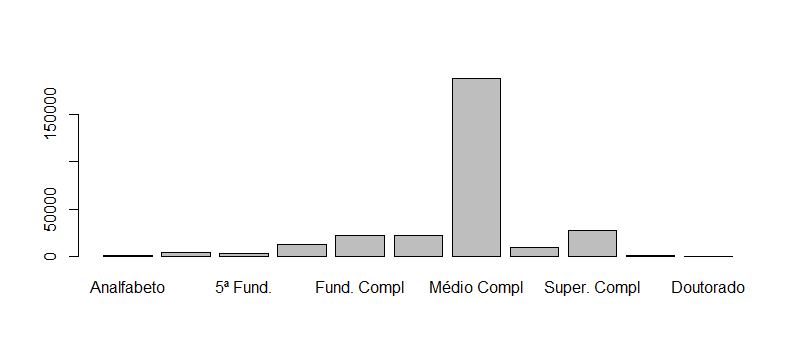
\includegraphics[width=1.0\textwidth]{Instrucao.png}
\caption{Grau de Instrução}
\label{fig:exampleFig10}
\end{figure}

\FloatBarrier
\begin{figure}[!htb]
\centering
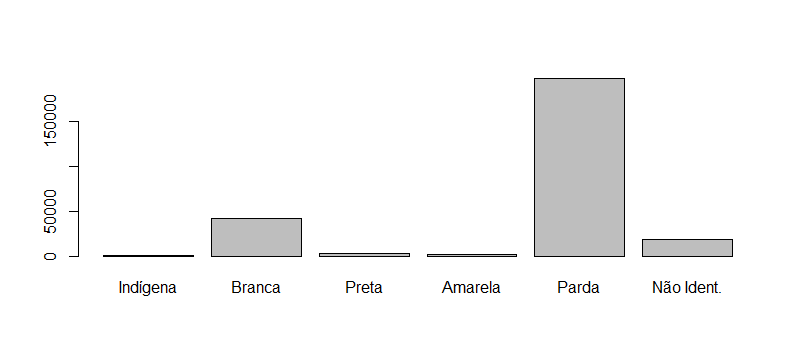
\includegraphics[width=1.0\textwidth]{Raca.png}
\caption{Raça / Cor}
\label{fig:exampleFig11}
\end{figure}

Esta circunstância poderá impactar em um peso maior na identificação das regras de associação. Avaliaremos se esta hipótese se confirma após realizarmos os experimentos desta pesquisa.

O comportamento da distribuição dos atributos alvo também aponta para uma concentração em alguma das possíveis categorias. Uma parcela considerável dos registros, cerca de XXX  apresenta a categorização de Sem Afastamento. Se o objetivo é verificar as relações existentes nos casos de afastamento será necessário filtrar estes dados.
No caso dos Desligamentos há uma maioria na categorização de Demissão sem justa causa, mas não com a mesma incidência que no caso dos afastamentos.

\FloatBarrier
\begin{figure}[!htb]
\centering
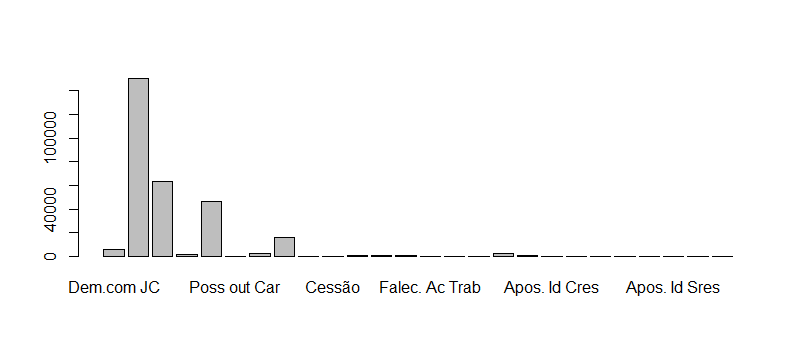
\includegraphics[width=1.0\textwidth]{Desligamento.png}
\caption{Desligamentos}
\label{fig:exampleFig3}
\end{figure}

\FloatBarrier
\begin{figure}[!htb]
\centering
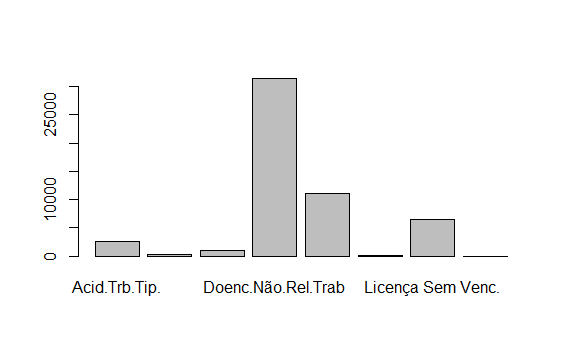
\includegraphics[width=0.7\textwidth]{Afastamento.png}
\caption{Afastamentos}
\label{fig:exampleFig4}
\end{figure}


\subsection{Pré- Processamento}

''Os Banco de Dados do mundo real de hoje são altamente suscetíveis a ruído, perdas e inconsistência de dados, além de serem tipicamente muito grandes e terem múltiplas, e heterogêneas fontes de origem. Baixa qualidade dos dados leva a baixa qualidade de resultados de mineração de dados."\cite{Han2012}
Desta forma faz-se necessário verificar a necessidade e alternativas de atuar sobre os dados. 

As ações de Pré-Processamento de Dados realizadas neste caso foram relativas a Limpeza de Dados, Redução dos Dados e Adaptações nas Observações. \cite{elmasri2015fundamentals}

\subsubsection{Limpeza de dados}    

Como nossos atributos alvo são afastamentos e desligamentos, os registros de nossa Base de Dados que não possuam preenchimento de informações em nenhum destes atributos devem ser eliminados. Não fazem parte do escopo de nossa pesquisa, neste momento.
Esta ação impactou na redução de 901.720 registros para 332.773 em nossa base.

\subsubsection{Redução de dados}

Como o arquivo original da RAIS continha 45 atributos e a nossa pesquisa abrangeria a ação de apenas 10 destes foi realizada uma Redução de dimensionalidade para que os atributos sem relevância para o Cesteh fossem desconsiderados em nossos experimentos.
Restaram apenas os atributos de desligamento, afastamento, sexo, faixa etária, número de funcionários na empresa, tempo de serviço, CBO e Raça/Cor.


\subsubsection{Adaptações nas Observações}    
 
A estrutura original dos registros da RAIS prevê em um único registro até três afastamentos e um desligamento. Com o objetivo de verificar o impacto de cada ocorrência em separado, realizamos a operação de gerar, a partir de um único registro, um registro específico para cada ocorrência.

Por exemplo, se um registro A possui afastamento1 preenchido, afastamento2 preenchido, iremos gerar então dois registro destintos com apenas um atributo de afastamento.

\subsubsection{Classificação Brasileira de Ocupação (CBO}

A Composição do código da CBO é de cinco dígitos, representando a seguinte estrutura e quantidades :

 1 - 10 Grandes Grupos
 2 - 47 Subgrupos Principais
 3 - 192 Subgrupos
 4 - 596 Grupos de Base
 5 - 2422 Ocupações
 
 Consideraremos uma visão por Subgrupo para a CBO para reduzir a dimensionalidade dos dados a serem avaliados.

\subsection{Dados da RAIS de 2015 no estado do Amazonas}

Após as operações de pré-processamento chegou-se uma distribuição de atributos por categoria modificada para as informações contidas no arquivo da RAIS de 2015 para o Amazonas.

Podemos destacar um equilíbrio na distribuição pelas categorias de número de funcionários da empresa e em pelo menos quatro opções da Classificação Brasileira de Ocupação (CBO). Há uma categoria que se destaca em Grau de Instrução, com predominância significativa dos que possuem Ensino Médio Completo e da Raça Parda. Sessenta por cento dos trabalhadores são do sexo Masculino e um terço deles possuem entre 30 e 39 anos. 

\FloatBarrier
\begin{figure}[!htb]
\centering
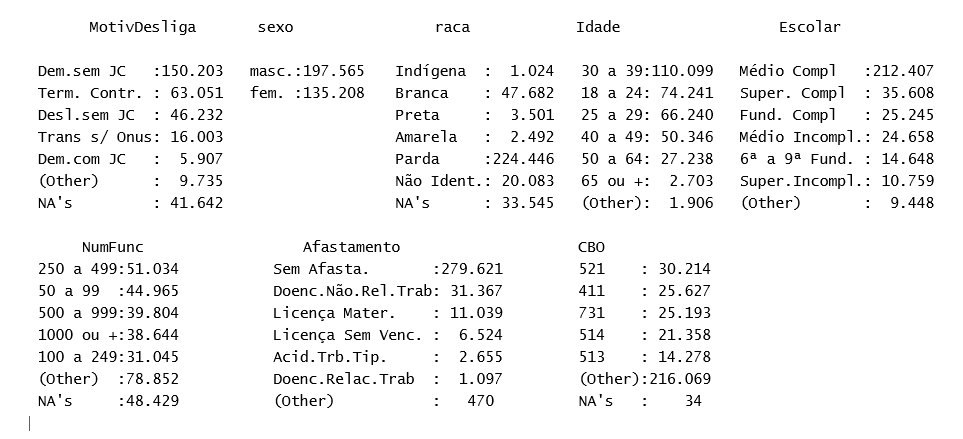
\includegraphics[width=1.1\textwidth]{resultado_base.png}
\caption{Dados de 2015 no Amazonas}
\label{fig:exampleFig5}
\end{figure}

\section{Metodologias de Mineração de Dados} 

Mineração de Dados deveria ser melhor nomeado como Mineração de Conhecimento a partir de dados. Várias são as abordagens de extração de conhecimento. Devido ao objetivo desta pesquisa  precisamos identificar relações entre os atributos de Afastamentos e os demais atributos, e o mesmo em relação aos Desligamentos. Optamos por identificação de RAs (Regras de Associação) utilizando o conceito de identificação de Padrões Frequentes.

\subsection{Padrões Frequentes}

Padrões Frequentes é um método de se minerar conhecimento procurando por padrões recorrentes. As associações e correlações entre os atributos envolvidos irão identificar padrões escondidos.\cite{james2014introduction}
Existem várias técnicas diferentes de se minerar padrões frequentes. Utilizaremos o algoritmo Apriori.\cite{agrawal1994fast}


\subsection{Algoritmo Apriori}

O Algoritmo Apriori  visa identificar Regras de Associação, ou seja, encontrar elementos que implicam na presença de outros elementos numa mesma transação. Há um princípio básico deste algoritmo que apoia este objetivo: Qualquer subconjunto de um conjunto de itens frequentes devem ser frequentes.\cite{Han2012}

Suporte e Confiança são medidas parametrizáveis de condições para execução do Apriori. Suporte mede a probabilidade da transação envolver a união entre os dois atributos, enquanto a confiança mede a probabilidade de caso um ocorra, o outro ocorra também. Os ajustes nos valores de suporte e confiança acarretam resultados diferentes na identificação das regras de associação.

Uma medida resultante, que relaciona confiança e suporte é a lift.\cite{Han2007} A importância da lift é que se o valor da mesma é menor que 1 isto sinaliza que não a associação entre as mesmas é fraca. Quanto maior que 1 ela for mais representativa é a associação entre os atributos. Por exemplo, um valor de lift de 1,83  entre os atributos A e B indica uma forte correlação entre eles, portanto se A ocorre existe uma chance 83 por cento maior de que B ocorra.  

A lógica do algoritmo pode ser representada por um pseudo-código.
\FloatBarrier
\begin{figure}[!htb]
\centering
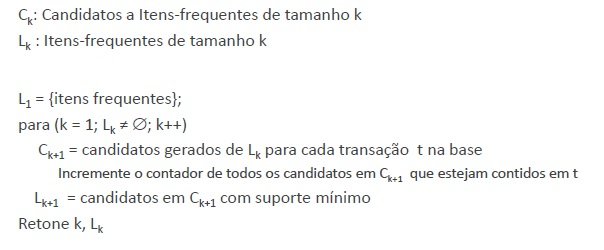
\includegraphics[width=0.9\textwidth]{PseudoCodigoApriori.jpg}
\caption{Algoritmo Apriori}
\label{fig:exampleFig12}
\end{figure}


\section{Experimentos Realizados}

Algumas opções de parametrização dos valores de suporte e confiança foram testados para identificar quais valores nos gerariam uma saída contendo um número de regras de associação que nos permitisse avaliar o comportamento desejado.

Por exemplo , quando executamos com um parâmetro de confiança igual a 0.9 para os desligamentos, foram geradas apenas 3 regras e nenhuma delas envolvendo o atributo alvo. Por outro lado, quando aumentamos a condição de suporte para 0.5, foram geradas 212 regras, o que prejudicou consideravelmente a avaliação.

A parametrização que gerou os resultados que apresentaremos nesta pesquisa foi de  Suporte = 0,1 e Confiança = 0,5.

\subsection{Resultados Afastamentos}

O total de registros processados na execução relativa aos afastamentos foi de 332.773 observações.
O valores mínimos de suporte foi de 0.10001, bem próximo ao valor do parâmetro, e variou até o valor máximo de 0.6629, evidenciando uma boa variação.

O valor mínimo de confiança foi de 0.5158, também próximo ao parâmetro, no entanto o valor máximo foi de 1.0000. Este valor deve ser avaliado com bastante atenção pois indica uma relação de 100 por cento dos casos para os atributos relacionados.
A relação que gerou a confiança de 100 por cento é entre os atributos sexo = feminino e afastamento por licença maternidade. Desta forma está justificado o resultado que o modelo gerou.

Os resultados de lift mostram que houve regras de saída que não indicavam uma forte relação de associação, visto que o valor mínimo apontado foi de 0.874, ou seja, menor que 1. Todavia foi registrado valor de lift máximo de 1.813, casos com aumento de 81 por cento  de casos em uma relação.

Sobre as regras apontadas com valores mais altos de confiança, considerando as 5 mais bem ranqueadas, vimos que a de mais alto valor foi a já avaliada anteriormente. Dentre as demais destacam-se as que relacionam com os afastamentos e os demais atributos com considerável incidência na base: raça parda, nível de instrução ensino médio completo, sexo masculino e idade entre 30 e 39 anos. Vale ressaltar no entanto que houve diferenciação entre o afastamentos relacionados, o que deve ser considerado na avaliação de possíveis regras de associação.

\FloatBarrier
\begin{figure}[!htb]
\centering
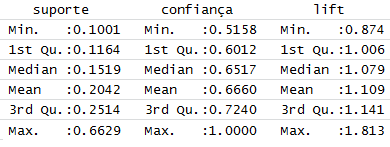
\includegraphics[width=0.8                                          \textwidth]{Sumary_Result_Afasta.png}
\caption{Sumário dos Afastamentos}
\label{fig:exampleFig6}
\end{figure}

\FloatBarrier
\begin{figure}[!htb]
\centering
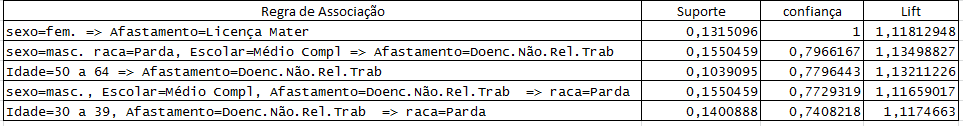
\includegraphics[width=1.0\textwidth]{top5_Afastamento.png}
\caption{Exemplo dos Resultados dos Afastamentos}
\label{fig:exampleFig7}
\end{figure}


\subsection{Resultados Desligamentos}

O total de registros processados na execução relativa aos afastamentos foi de 291.131 observações.
O valores mínimos de suporte foi de 0.1022, bem próximo ao valor do parâmetro, e variou até o valor máximo de 0.6799, evidenciando uma boa variação e quase idêntico ao encontrado no processamento dos afastamentos.

O valor mínimo de confiança foi de 0.5104, mais uma vez próximo ao encontrado nos afastamentos, no entanto o valor máximo desta vez foi de 0.7373, que não indica nenhuma questão bem específica e rara.

Os resultados de lift mostram que com os desligamentos também ocorreram regras com valores menores que 1, mas o que chama mais atenção neste caso é a ocorrência de um valor máximo de 2.599, indicando uma relação de alta associação entre os atributos.
A situação em questão envolve os atributos de tempo de empresa igual a 1 ano e o desligamento por término de contrato. Podemos avaliar que há muitos contratos cujo prazo de validade seja de 1 ano ou menos que 2 anos,e que ao término destes ocorra um desligamento, já previsto pelo término do contrato.

Em relação aos desligamentos relacionamos em destaque as 5 mais bem ranqueadas, mas que envolvam necessariamente um atributo alvo.
O resultado demonstra claramente o destaque para o desligamento por demissão sem justa causa. Isto se deve ao fato de que um percentual de 47 por cento das ocorrências de desligamento sejam por este motivo. A única que aparece com um atributo alvo diferente é justamente a que possui alto valor de lift.


\FloatBarrier
\begin{figure}[!htb]
\centering
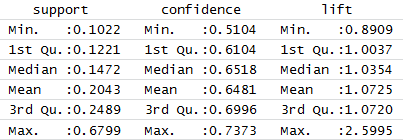
\includegraphics[width=0.8\textwidth]{Sumary_Desligamento.png}
\caption{Sumário dos Desligamentos}
\label{fig:exampleFig8}
\end{figure}

\FloatBarrier
\begin{figure}[!htb]
\centering
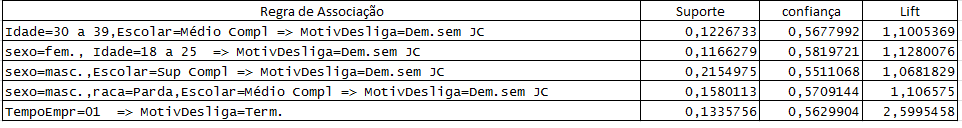
\includegraphics[width=1.0\textwidth]{top5Desligamento.png}
\caption{Exemplo dos Resultados dos Desligamentos}
\label{fig:exampleFig9}
\end{figure}


\section{Considerações Finais}

Após a realização dos experimentos relacionados e dos resultados obtidos podemos chegar a algumas conclusões e também indicações relevantes de continuidade deste trabalho.

\subsection{Conclusões}

O uso de padrões frequentes  mostrou ser uma ferramenta útil na identificação de associações entre os dados  e o grau de dependência entre os mesmos ao ser aplicada na base da dados da RAIS.  

Podemos confirmar a hipótese inicial de que algumas das associações obtiveram destaque em razão do significativo  volume de dados de determinado atributo.

Existem inúmeras demandas do CESTEH que seriam atendidas com a aplicação de padrões frequentes, e outras técnicas de Mineração de Dados. 


\subsection{Trabalhos Futuros}

O aprendizado com a experiência desta pesquisa nos permitiu perceber uma gama considerável de alternativas de continuidade para este trabalho.
Relacionamos algumas delas, sinalizando a real intenção de dar sequência a esta pesquisa:

\begin{itemize}
    \item Realizar os experimentos deste trabalho para o ano de 2015 abrangendo todas as Unidades da Federação.
    \item Realizar os experimentos deste trabalho com os algoritmos com os algoritmos FP-Tree e ECLAT, de padrões frequentes. 
    \item Realizar agrupamentos dos afastamentos e dos desligamentos por CBO, utilizando k-means.
    \item Identificar regras de associações apenas entre afastamentos e desligamentos, sem incluir outros atributos.
    
\end{itemize}

\section{References}


\bibliographystyle{sbc}
\bibliography{ivaluques.bib}

\end{document}
